\begin{english}

\chapter{Implementing Web-based Visualizations}
\label{cha:web_based_visualization}

Web-based Visualization has a long history in Scientific Visualization and Information Visualization and has seen a recent resurgence in the larger context of social visualization~\cite{Johnson08}. These visualizations have been realized using small applets which are backed by programming environments such as Adobe Flash or Java. With the latest progression of browser technology, these third-party applets are continuously replaced with web-native API's. This chapter gives an overview about techniques and tools available for building interactive web-based visualizations.

According to Bostock and Heer~\cite{Protovis09}, tools used to visualize data are divided into two categories: 
\emph{Visualization Systems} are high-level abstractions that are primarily used for data visualization, whereas \emph{Graphical Systems} operate on low-level graphical primitives. This dichotomy is not meant to be seen as strict. Thus, toolkits may fall somewhere in between.

\section{Graphical Systems}
%%%-----------------------------------------------------------------------------

Low-level graphical systems have a long history in computer science. They are ranging from vector-based drawing programs (e.g. Adobe Illustrator) to low-level rendering API's (OpenGL, Java2D and Processing)~\cite{Protovis09}. Drawing programs aim to improve accessibility and allow designers to manipulate graphical marks in order to build and customize their visualizations. However those drawings are mostly static and demand manual composition by the designer.

In order to support interactive visualizations, which are generated based on live data, the usage of Rendering API's is necessary. In addition to traditional API's (OpenGL, Java2D), modern languages, such as Processing, have been developed to make the process of creating visualizations easier. Processing provides a simplified interface and enables even non-programmers to construct visualizations.

These libraries are general purpose, but typically support only imperative methods for rendering graphical primitives such as ellipses and polygons~\cite{Protovis09}. In response to that, higher-level tools such as Flash and Piccolo were introduced to simplify tasks such as \emph{interaction} and \emph{animation} by providing a \emph{scene graph} abstraction. All those API's do not provide any visualization abstractions, thus tasks such as layouting, interaction, animation (motion-tweening) are left to the user.


\section{Visualization Systems}
%%%-----------------------------------------------------------------------------

According to Bostock and Heer~\cite{Protovis09}, Visualization Systems are tools explicitly designed for the purpose of data visualization. They include common abstractions and mathematical models to make the task of creating interactive visualizations easier. Such tools include support for \emph{data-management}, \emph{layout algorithms}, \emph{interaction}, and \emph{animation}.


\subsection{Consumer Software}
%%%-----------------------------------------------------------------------------

The most widely-used visualization tools are built into consumer software, such as spreadsheet applications like Microsoft Excel or Google Spreadsheets. Such tools typically take tabular data as their input and map it to a visual representation based on a user-selected chart-type. Those tools are easy to use and have broad success, although there are a number of shortcomings, noted by Wilkinson~\cite{wilkinson2005grammar}.
Users only have limited options to adjust the built-in chart types and they cannot introduce new ones. According to Bostock and Heer, due to the high cost of switching tools and the iterative nature of visualization design~\cite{card99}, frequent compromise is likely.

\subsection{Analytical and Exploratory Tools}
%%%-----------------------------------------------------------------------------

A second category are \emph{Analytical and Exploratory Tools}, which are designed to provide flexible options for visual data explorations. A prominent example is Tableau\footnote{http://www.tableausoftware.com/}, which integrates data manipulation with visualization. Tableau allows to adjust queries by interacting with the visual representation. Other approaches, such as Wilkinson's Grammar of Graphics \cite{wilkinson2005grammar}, a dedicated language for specifying visualizations as statistical graphs, offer greater flexibility. Such systems take advantage of meta-data in order to derive appropriate default visual encodings \cite{Bertin83,Mackinlay86automatingthe}.

According to Heer and Bostock, control over graphical output is still limited for these tools. Also, they form closed systems, making them unsuitable for the design of customized domain specific visualizations~\cite{Protovis09}.


\subsection{Programming Toolkits}
%%%-----------------------------------------------------------------------------

The third category identified by Bostock and Heer are \emph{Programming Toolkits}, which are popular for presenting live data or allowing user interaction. While some of them (e.g. Google Chart API\footnote{http://code.google.com/apis/chart/}) only support a number of chart types, thus implying similar trade-offs as consumer software, others are more expressive and extensible (such as the InfoVisToolkit\footnote{http://thejit.org/} or Flare\footnote{http://flare.prefuse.org/}). These tools typically come with a data management framework, coupled with visualization and interaction components.

The InfoVis Toolkit, for example, introduces ``widgets'' that combine visualizations into separate units, which can be extended at any time. In contrast, Prefuse and Flare follow the data state model \cite{Chi98anoperator} and maintain a collection of parametrized visual objects, each associated with data. Using this approach, designers are enabled to specify the properties of visual objects (e.g. position, shape, color) by using configurable operators in order to determine layout and color encoding. 

Protovis~\cite{Protovis09}, the proposed solution by Bostock and Heer, introduces a declarative specification allowing the separation of \emph{specification} and \emph{execution}. The declarative specification is portable, so additional rendering engines such as Java2D or Flash can be targeted in future. Also, this approach should allow the optimization of the visualization pipeline, for example through lazy evaluation of visual properties with large datasets.


\section{Available Technology} % The web as an environment
%%%-----------------------------------------------------------------------------

Although creating graphically intensive applications was already possible with 3rd-party browser plugins, such as Java Applets, Adobe Flash or Microsoft Silverlight, several native visualization methods are available today. These allow the creation of interactive visualizations directly in the browser without requiring any third-party dependencies. This section describes the most important technologies that are available in current web browsers.

\subsection{SVG}
%%%-----------------------------------------------------------------------------

SVG (Scaleable Vector Graphics) is an earlier standard for drawing shapes in browsers recommended by the World Wide Web Consortium (W3C). SVG is a higher level graphical system providing an interface to an underlying scene graph, which is subsequently rendered to a bitmap. Users can manipulate attributes of certain objects by interacting with the Document Object Model (DOM) interface. Once attributes have been changed, SVG can automatically re-render parts of the scene. The SVG API enables events to be associated with objects, so users can bind event handlers to certain events, e.g. when the user clicks on a certain rectangle. The SVG scene graph can be represented in XML, which serves as an exchange format. SVG has a number of built-in simple shapes, such as rectangles and circles. For more complex shapes, users can utilize SVG's path element.

Because SVG can be represented as XML, external editors can be used to design graphical objects, which are composed of primitive SVG-shapes. Those graphical objects can be injected into an existing SVG scene graph, which provides some sort of modularization.

\subsection{HTML5 Canvas}
%%%-----------------------------------------------------------------------------

The Canvas Element is part of the HTML5 specification\footnote{http://dev.w3.org/html5/spec/Overview.html} and allows dynamic, scriptable rendering of 2D shapes and bitmap images. Canvas uses immediate mode rendering with graphical elements drawn as Javascript commands are issued. Canvas is memory efficient, because only the initial data-structures and the rasterized pixels must be stored in memory. Thus, Canvas is able to display a huge amount of objects, while keeping the memory footprint low. An equivalent SVG representation would consume more memory, as each object of the scene graph must be stored. Conceptually, the Canvas API is a lower level protocol and does not offer a scene graph, but a pixel buffer which can be manipulated by the user.

Since Canvas does not maintain graphical objects, hit testing, which is needed for implementing interaction, must be done manually by matching the coordinates of the mouse click with the coordinates of the drawn shape to determine whether it was clicked, or not.


\subsection{Javascript}
%%%-----------------------------------------------------------------------------

The programming language of the web is \emph{Javascript}. While established platforms (e.g. Java, C, C++) provide a vast number of supportive libraries, the availability of such libraries is rather limited for client-side Javascript. In terms of performance, current Javascript implementations are sufficiently fast. Modern browsers even allow parallel processing through WebWorkers. Because of the nature of the language (interpreted, prototypical, functional), it is questionable if the same programming patterns (familiar from classical environments) should be applied. Javascript developers are increasingly preferring declarative interface design to imperative programming style. The expressive power of domain specific languages (DSL) is also realized frequently and fits well into the Javascript programming model \cite{deursen2000}. A DSL is a higher level abstraction focussing on a particular application domain and providing a simplified interface. In the context of Information Visualization, it seems reasonable to apply those modern patterns to visualization toolkits and supportive libraries as well.

\section{Tools Landscape}
%%%-----------------------------------------------------------------------------

Based on recent developments in the field of web-based Information Visualization, a selection of established visualization libraries is introduced. It will be examined which approaches they follow, what type of application they are intended for and how they differ from each other. For illustration, each toolkit will be utilized to construct a simple barchart in order to show differences in usage.


\subsection{Processing.js}
%%%-----------------------------------------------------------------------------

Processing.js is a port of the Processing Visualization Language, originally developed by Ben Fry and Casey Reas. It allows existing Processing code to be executed in a web-based environment, powered by the HTML5 Canvas element. It can be used for specifying visualizations in a classical imperative programming style. In order to support native Processing.js code, which is specified in Java syntax, a source code compilation step is necessary. If a user wants to use a widely-adopted visualization language and be able to execute it on the web, or reuse existing Processing code, Processing.js might be a good choice. However, if visualizations are built from scratch and just target the web-platform for execution, there might be better options. Especially the imposed source-code transformation step might complicate debugging and interacting with web-native API's. Processing.js requires users to specify data-types (this is because it uses Java syntax), which is superfluous as Javascript itself is an untyped prototypal language.

In Processing, users might specify a bar chart as a series of rectangles using a for loop and a call to \texttt{rect()}, which immediately draws a single bar to the canvas:

\begin{verbatim}
int[] data = {1, 1.2, 1.7, 1.5, .7, .3};
for (int i = 0; i < data.length; i++) {
  fill(0, 0, 255);
  rect(i * 25, 200, 20, -data[i] * 80);
}
\end{verbatim}


\subsection{Protovis}
%%%-----------------------------------------------------------------------------

Protovis is an extensible toolkit for constructing visualizations by composing simple graphical primitives. In Protovis, designers specify visualizations as a hierarchy of marks with visual properties defined as functions of data. This representation achieves a level of expressiveness comparable to low-level graphics systems, while improving efficiency (the effort required to specify a visualization) as well as accessibility (the effort required to learn and modify the representation).

Protovis is similar to other graphics libraries such as Java 2D or Processing. It provides a mechanism for drawing rectangles (bars), circles (dots), lines, and polygons (areas). However, Protovis uses a declarative rather than imperative syntax. In contrast to Processing.js, Protovis users almost never use a loop. A set of related graphical elements, such as the bars in a bar chart, are specified as a single mark. The mark is associated with data and the properties are specified as functions, encoding the data graphically:

\begin{verbatim}
vis.add(pv.Bar)
  .data([1, 1.2, 1.7, 1.5, .7, .3])
  .width(20)
  .height(function(d) { return d * 80 })
  .bottom(0)
  .left(function() { return this.index * 25});
\end{verbatim}

\SuperPar When it comes to animation, Protovis allows to specify transitions, but it turned out there are critical limitations. That is why this project was discontinued in favor of D3.js, the official successor of Protovis, which uses a fundamentally different approach, targeting animation and interaction~\cite{D3}.


\subsection{D3.js}
%%%-----------------------------------------------------------------------------

D3 (Data-Driven Documents)~\cite{D3} is a progression of Protovis, developed by its original author, Michael Bostock. Instead of using an execution independent specification language, D3 enables direct inspection and manipulation of a web-native representation: the standard Document Object Model (DOM). With D3, designers selectively bind input data to document elements, which are part of the DOM. They are applying dynamic transforms to do both, generate and modify content. Using an representation transparent approach, expressiveness can be improved and the immediate evaluation of operators simplifies debugging and allows iterative development. The downside of this is that D3 is tied to a specific representation, the DOM, and thus cannot be ported to another rendering engine. D3 was built for the purpose of animation to allow highly interactive and responsive data visualizations. The specification of a bar chart would read as follows:

\begin{verbatim}
var bars = vis.selectAll("g")
    .data([1, 1.2, 1.7, 1.5, .7, .3])
  .enter().append("svg:g")
    .attr("transform", function(d, i) {
      return "translate(" + i*25 + ", 0)"; 
    });
bars.append("svg:rect")
    .attr("width", 20)
    .attr("height", function(d) { return d * 80; });
\end{verbatim}


\subsection{Unveil.js}
%%%-----------------------------------------------------------------------------

Unveil.js, the toolkit developed in the course of this thesis, implements a higher level visualization framework on top of HTML5 Canvas. It introduces graphical objects, adds an API for specifying animations and provides mechanisms to reduce overall CPU consumption. In other words, it tries to unite the advantages of both interfaces, SVG and Canvas. Chapter~\ref{cha:unveil} covers this in more detail.

\begin{verbatim}
var scene = new uv.Scene({
  actors: function() {
    return _.map([1, 1.2, 1.7, 1.5, .7, .3], function(d, index) {
      return {
        type: 'rect',
        x: index * 25,
        y: 200,
        width: 20,
        height: -d * 80,
        fillStyle: 'blue'
      }
    });
  }();
});
\end{verbatim}



\subsection{VVVV.js}
%%%-----------------------------------------------------------------------------

VVVV is a graphical programming environment for prototyping and developing multi-media applications and interactive visualizations. While the original VVVV runs as a desktop application on Windows, VVVV.js\footnote{http://vvvvjs.quasipartikel.at} introduces a web-based runtime environment for VVVV patches. VVVV.js is a work-in-progress, but introduces a novel approach to web-based data visualization. Visualizations are no longer specified as literal source code, but using a visual programming language, expressed through nodes that are connected by input and output pins. Nodes function as independent modules, which take input data, do some processing and yield output data accordingly. The implementation of a node forms a single instruction that operates on multiple data items. In addition to artistic targets, VVVV.js can also be utilized efficiently for creating data visualizations. Figure~\ref{fig:vvvvjs} shows the specification of the barchart example.

\begin{figure}
\centering
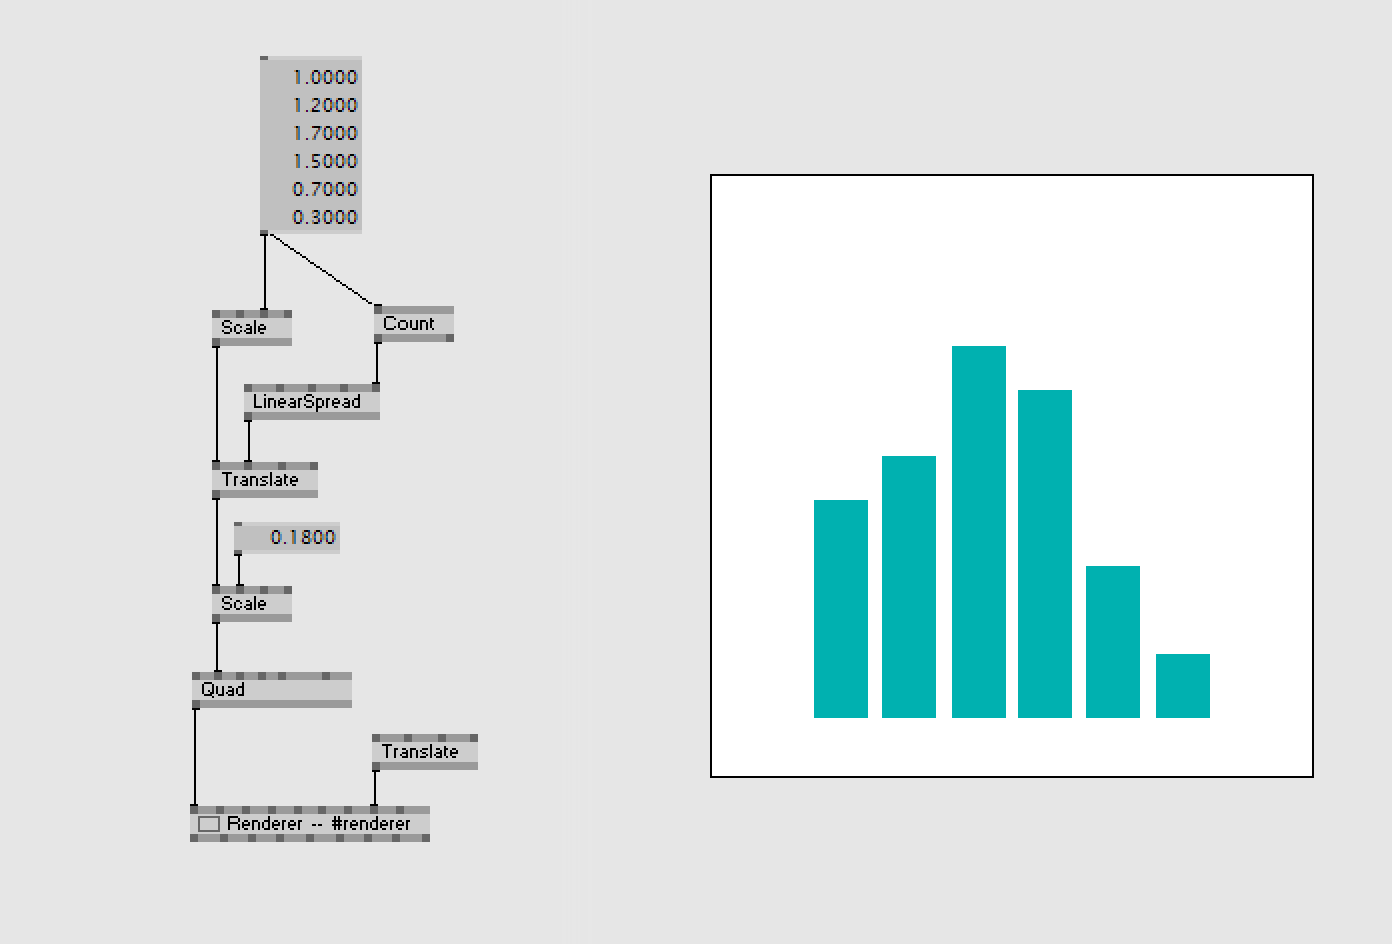
\includegraphics[width=1\textwidth]{vvvvjs}
\caption{VVVV.js used to visually specify a simple Barchart}
\label{fig:vvvvjs}
\end{figure}


\section{Summary}
%%%-----------------------------------------------------------------------------

It is quite hard to choose the right technology for a certain visualization task. If there are huge amounts of data involved, web-native solutions may be exhausted, thus relying on classical environments may remain a better choice. If the requirements on data transmission are suitable for the web, it depends on the task and the favored approach of the developer, which native technology should be utilized. Browsers use different implementations and support different aspects of these technologies. 

However, SVG as well as HTML5 Canvas are thoroughly supported by the majority of current web browsers. After looking at the current range of available toolkits, different approaches were identified such as \emph{toolkit-specific abstraction} vs. \emph{representation transparency} or \emph{imperative programming} vs. \emph{declarative specification}. These are all fundamentally different strategies to approach Information Visualization, each having its own field of application. It is important to understand these differences in order to choose the right tools to build efficient visualizations.

It must also be taken into account that in practice, developers often need to support legacy browsers, that do not support the new interfaces (e.g. Internet Explorer prior to Version 9 does not support the Canvas Element).

\end{english}